\chapter{Background}
\label{cha:bkg}
Literature Review

\section{Posture/Gesture Recognition}
\label{sec:pgr}
All the literature review I can borrow from the previous report.

a pattern or an object in a two-dimensional image can be described with four properties~\cite{wysoski2008fast}: position, geometry (size, area and shape), color and texture, and trajectory. Appearance-based methods are the most direct approaches to perform pattern recognition. 
The test image is compared with all the templates to find the best match on one particular or a combination of properties. 
In terms of classification algorithms, distance measure methods (nearest neighbour, k-means clustering), support vector machine (SVM), multi-layer perceptron (MLP) neural networks and statistical methods, e.g. Gaussian mixture model (GMM) have been applied successfully in visual recognition. 
Since the 2D projection of an object changes under various illuminations, viewing angles, relative positions and distances (size), it is impossible to represent all appearances of an object in different conditions. 
Robust matching methods are employed, such as edge matching~\cite{canny1986computational}, the divide-and-conquer approach~\cite{toygar2004multiple}, gradient matching~\cite{wei2006robust}, etc. 
Moreover, feature based methods are used to improve reliability, robustness and classification efficiency. 
Among various feature extraction methods, the scale-invariant feature transform (SIFT)~\cite{lowe2004distinctive} and the sped-up robust features (SURF)~\cite{bay2008speeded} methods are well-accepted recently in the field. 
However, to find a proper feature for a specific object still remains an open question and there is not any process as accurate, general and effective as the brain.
Turning to biology for answers is always the way to explore the field of visual pattern recognition. 
Riesenhuber and Poggio~\cite{riesenhuber1999hierarchical} presented a biologically-inspired model following the organization of the visual cortex which has the ability to represent relative position- and scale-invariant features. Integrating a rich set of visual features became available using a feed-forward hierarchical pathway. 

More and more attention has been drawn into the investigation of spiking neural networks for vision processing. 
Pattern information can be encoded in the delays between the pre- and post-synaptic spikes since the spiking neurons are capable of computing radial basis functions (RBFs)~\cite{hopfield1995pattern}.  
A further study~\cite{natschlager1998spatial} has stated that spatio-temporal information can be also stored in the exact firing time instead of the relative delay. Maass~\cite{maass1997networks} has proved mathematically that:
1) networks of spiking neurons are computationally more powerful than the first and second generation of neural network models;
2) a concrete biologically relevant function can be computed by a single spiking neuron, replacing  hundreds of hidden units in a sigmoidal neural net;
3) any function that can be computed by a small sigmoidal neural net can also be computed by a small network of spiking neurons.
Applications of SNN-based vision processing have been successfully carried out. 
A two-layered SNN has been trained using spike time dependent plasticity (STDP) and employed for a character recognition task~\cite{gupta2007character}. 
Lee and co-authors~\cite{6467270} have implemented the direction selective filters in real time using spiking neurons. 
The direction selective filters here are considered as a layer of convolution module in the model of so called convolution neural network~\cite{camunas2012event}. 
Different features, such as Gabor filter features (scale, orientation and frequency) and shape can be modelled as layers of feature maps. 
Rank order coding, as an alternative to conventional rate-based coding, treats the first spike the most important and has well applied to an orientation detection training process~\cite{delorme2001networks}. 
Nengo~\cite{eliasmith2011nengo} is a graphical and scripting based software package for simulating large-scale neural systems and has been used to build the world's largest functional brain model, Spaun~\cite{eliasmith2012large}. An FPGA implementation of a Nengo model for digit recognition has been reported~\cite{naylor2013managing}. 
Deep Belief Networks (DBNs), the 4th generation of artificial neural network, has shown a strong ability in solving classification problems. 
A recent study~\cite{o2013real} has resoundingly mapped an offline-trained DBN onto an efficient event-driven spiking neural network for a digit recognition task.
Hand segmentation and feature extraction usually takes the colour into account and involves wavelets, e.g. using a Kalman filter. 
Thus, shape-only recognition of the hand posture will be a challenge. 
In the terms of gesture recognition, the hidden Markov model (HMM) has shown its ability to recognize dynamic gestures~\cite{elmezain2009hidden}. 
However, with their instinctive temporal processing, SNNs have the potential to deliver dynamic gesture recognition.



\section{Biology Aspect}
\label{sec:bio}
A lot to work on this part.
May or may not include neuron models.

\section{Platforms}
\label{sec:plt}

\textcolor{blue}{
This section presents some details of the two hardware components, the Address-Event Representation (AER) silicon retina~\cite{lenero20113} and the SpiNNaker system~\cite{furber2014spinnaker} which is a massive parallel computing platform aimed at real-time simulation of spiking neural networks (SNNs). 
Figure~\ref{fig:SysOverView} shows the combined hand posture recognition system; 
the AEREAR2 silicon retina connected to the SpiNNaker 48-node board via a Spartan 6 FPGA board~\cite{galluppi2012real}.%, which was also applied to a sound localisation system.
The jAER~\cite{delbruck2008frame} event-based processing software\footnote{\url{http://sourceforge.net/p/jaer/wiki/Home/}} running on the PC configures the retina and displays the output spikes through a USB link.
The host communicates to the SpiNNaker board via Ethernet to set up its runtime parameters and to download the neural network model off-line and uses a visualiser~\cite{6252490} to show the spiking activities in real-time.
}

\begin{figure}
\centering
	\begin{subfigure}[t]{0.6\textwidth}
		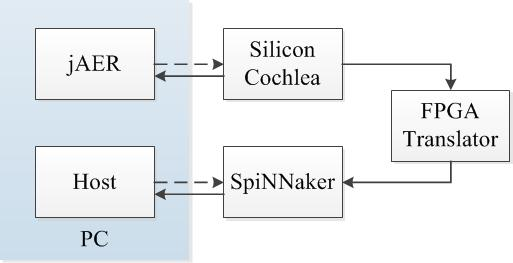
\includegraphics[width=\textwidth]{pics/outline.jpg}
	    \caption{Outline of the platform}
	    \label{fig:SysOverViewa}
	\end{subfigure}
	\\
	\begin{subfigure}[t]{0.6\textwidth}
		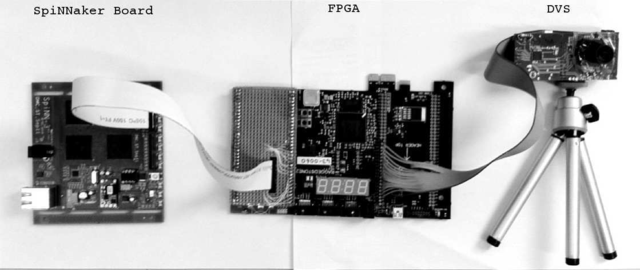
\includegraphics[width=\textwidth]{pics/dvs_spinnaker.png}	    \caption{Picture of the hardware platform}
	    \label{fig:SysOverViewb}
	\end{subfigure}	

\caption{System overview of the posture recognition platform. The silicon retina connects to the SpiNNaker system through an FPGA board. 
Spikes from the retina are streamed to the SpiNNaker system through this Spartan-6 FPGA board.
The jAER software configures the retina and displays its outgoing spikes through the USB connection.
The host sets up the runtime parameters off-line and downloads the network model to the SpiNNaker system.
}
\label{fig:SysOverView}
\end{figure}

\subsection{Vision Processing Front-ends}
\textcolor{blue}{
The visual front-end is constituted by a Dynamic Video Sensor (DVS) silicon retina, an asynchronous sensor which provides spike events encod-
ing the address of pixels undergoing a contrast change\cite{wei2006robust}. 
This approach lies in opposition to the more traditional method of sending entire frames to provide fast (3 $\mu$s latency) data-driven contrast detection at a wide range of illuminations. 
The sensor is capable of transmitting from 1 Keps to 20 Meps (events per
second).}
\subsection{SNNs Back-ends}
The SpiNNaker project's architecture mimics the human brain's biological structure and functionality. 
This offers the possibility of utilizing massive parallelism and redundancy to provide resilience in an environment of unreliability and failure of individual components.

In the human brain, communication between its computing elements, or neurons, is achieved by the transmission of electrical "spikes" along connecting axons. 
The biological processing of the neuron can be modelled by a digital processor and the axon connectivity can be represented by messages, or information packets, transmitted between a large number of processors which emulate the parallel operation of the billions of neurons comprising the brain.

The engineering of the SpiNNaker concept is illustrated in the Figure~\ref{fig:sysdia} where the hierarchy of components can be identified. 
Each element of the toroidal interconnection mesh is a multi-core processor known as the "SpiNNaker Chip" comprising 18 processing cores. 
Each core is a complete processing sub-system with local memory and a DMA capability. 
It is connected to its local peers via a Network-on-Chip (NoC) which provides local high bandwidth communication and to other SpiNNaker chips via links between SpiNNaker chips. 
In this way the massive parallelism extending to thousands or millions of processors is possible.

\begin{figure}
\centering
	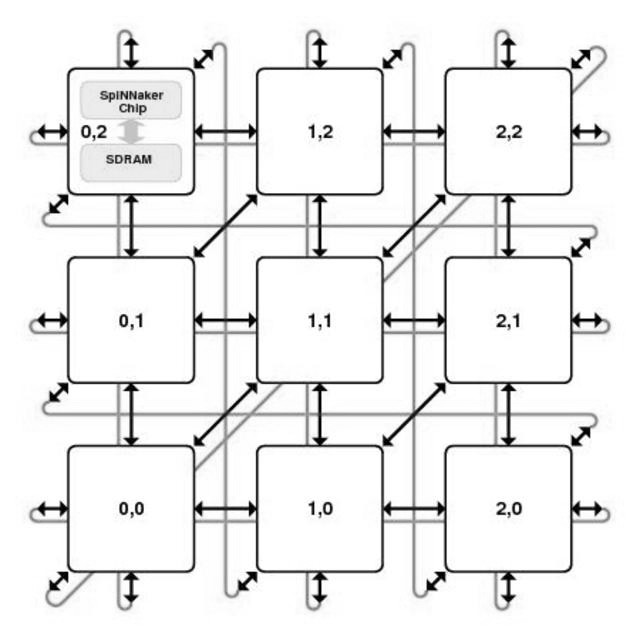
\includegraphics[width=0.6\textwidth]{pics/mesh_ctiff.jpg}
	\caption{System diagram}
	\label{fig:sysdia}
\end{figure}

The knowledge content and learning ability of the brain is embodied in its evolvable interconnection pattern; 
this routes a spike generated by one neuron to others which are interconnected with it by axons and these interconnections are modified and extended as a result of the learning and processes.

In SpiNNaker a packet Router within each multi-core processor controls the neural interconnection. 
Each transmitted packet representing a spike contains information which identifies its source neuron; 
this is used by a multi-core processor's Router to identify whether this packet should be routed to one of its contained application processors to respond, or should be routed on to one of the six adjacent multi-core processors connected to it as part of the overall SpiNNaker network.

The 103 machine is the 48-node board, see Figure~\ref{fig:48node}, and has 864 ARM processor cores, typically deployed as 768 application cores, 48 Monitor Processors and 48 spare cores. The 103 machine requires a 12V 6A supply. 
The control interface is two 100Mbps Ethernet connections, one for the Board Management Processor and the second for the SpiNNaker array. 
There are options to use the nine on-board 3.1Gbps high-speed serial interfaces (using SATA cables, but not necessarily the SATA protocol) for I/O; 
this will require suitable configuration of the on-board FPGAs that provide the high-speed serial interface support. 
103 boards can be connected together to form larger systems using the high-speed serial interfaces. 

\begin{figure}
\centering
	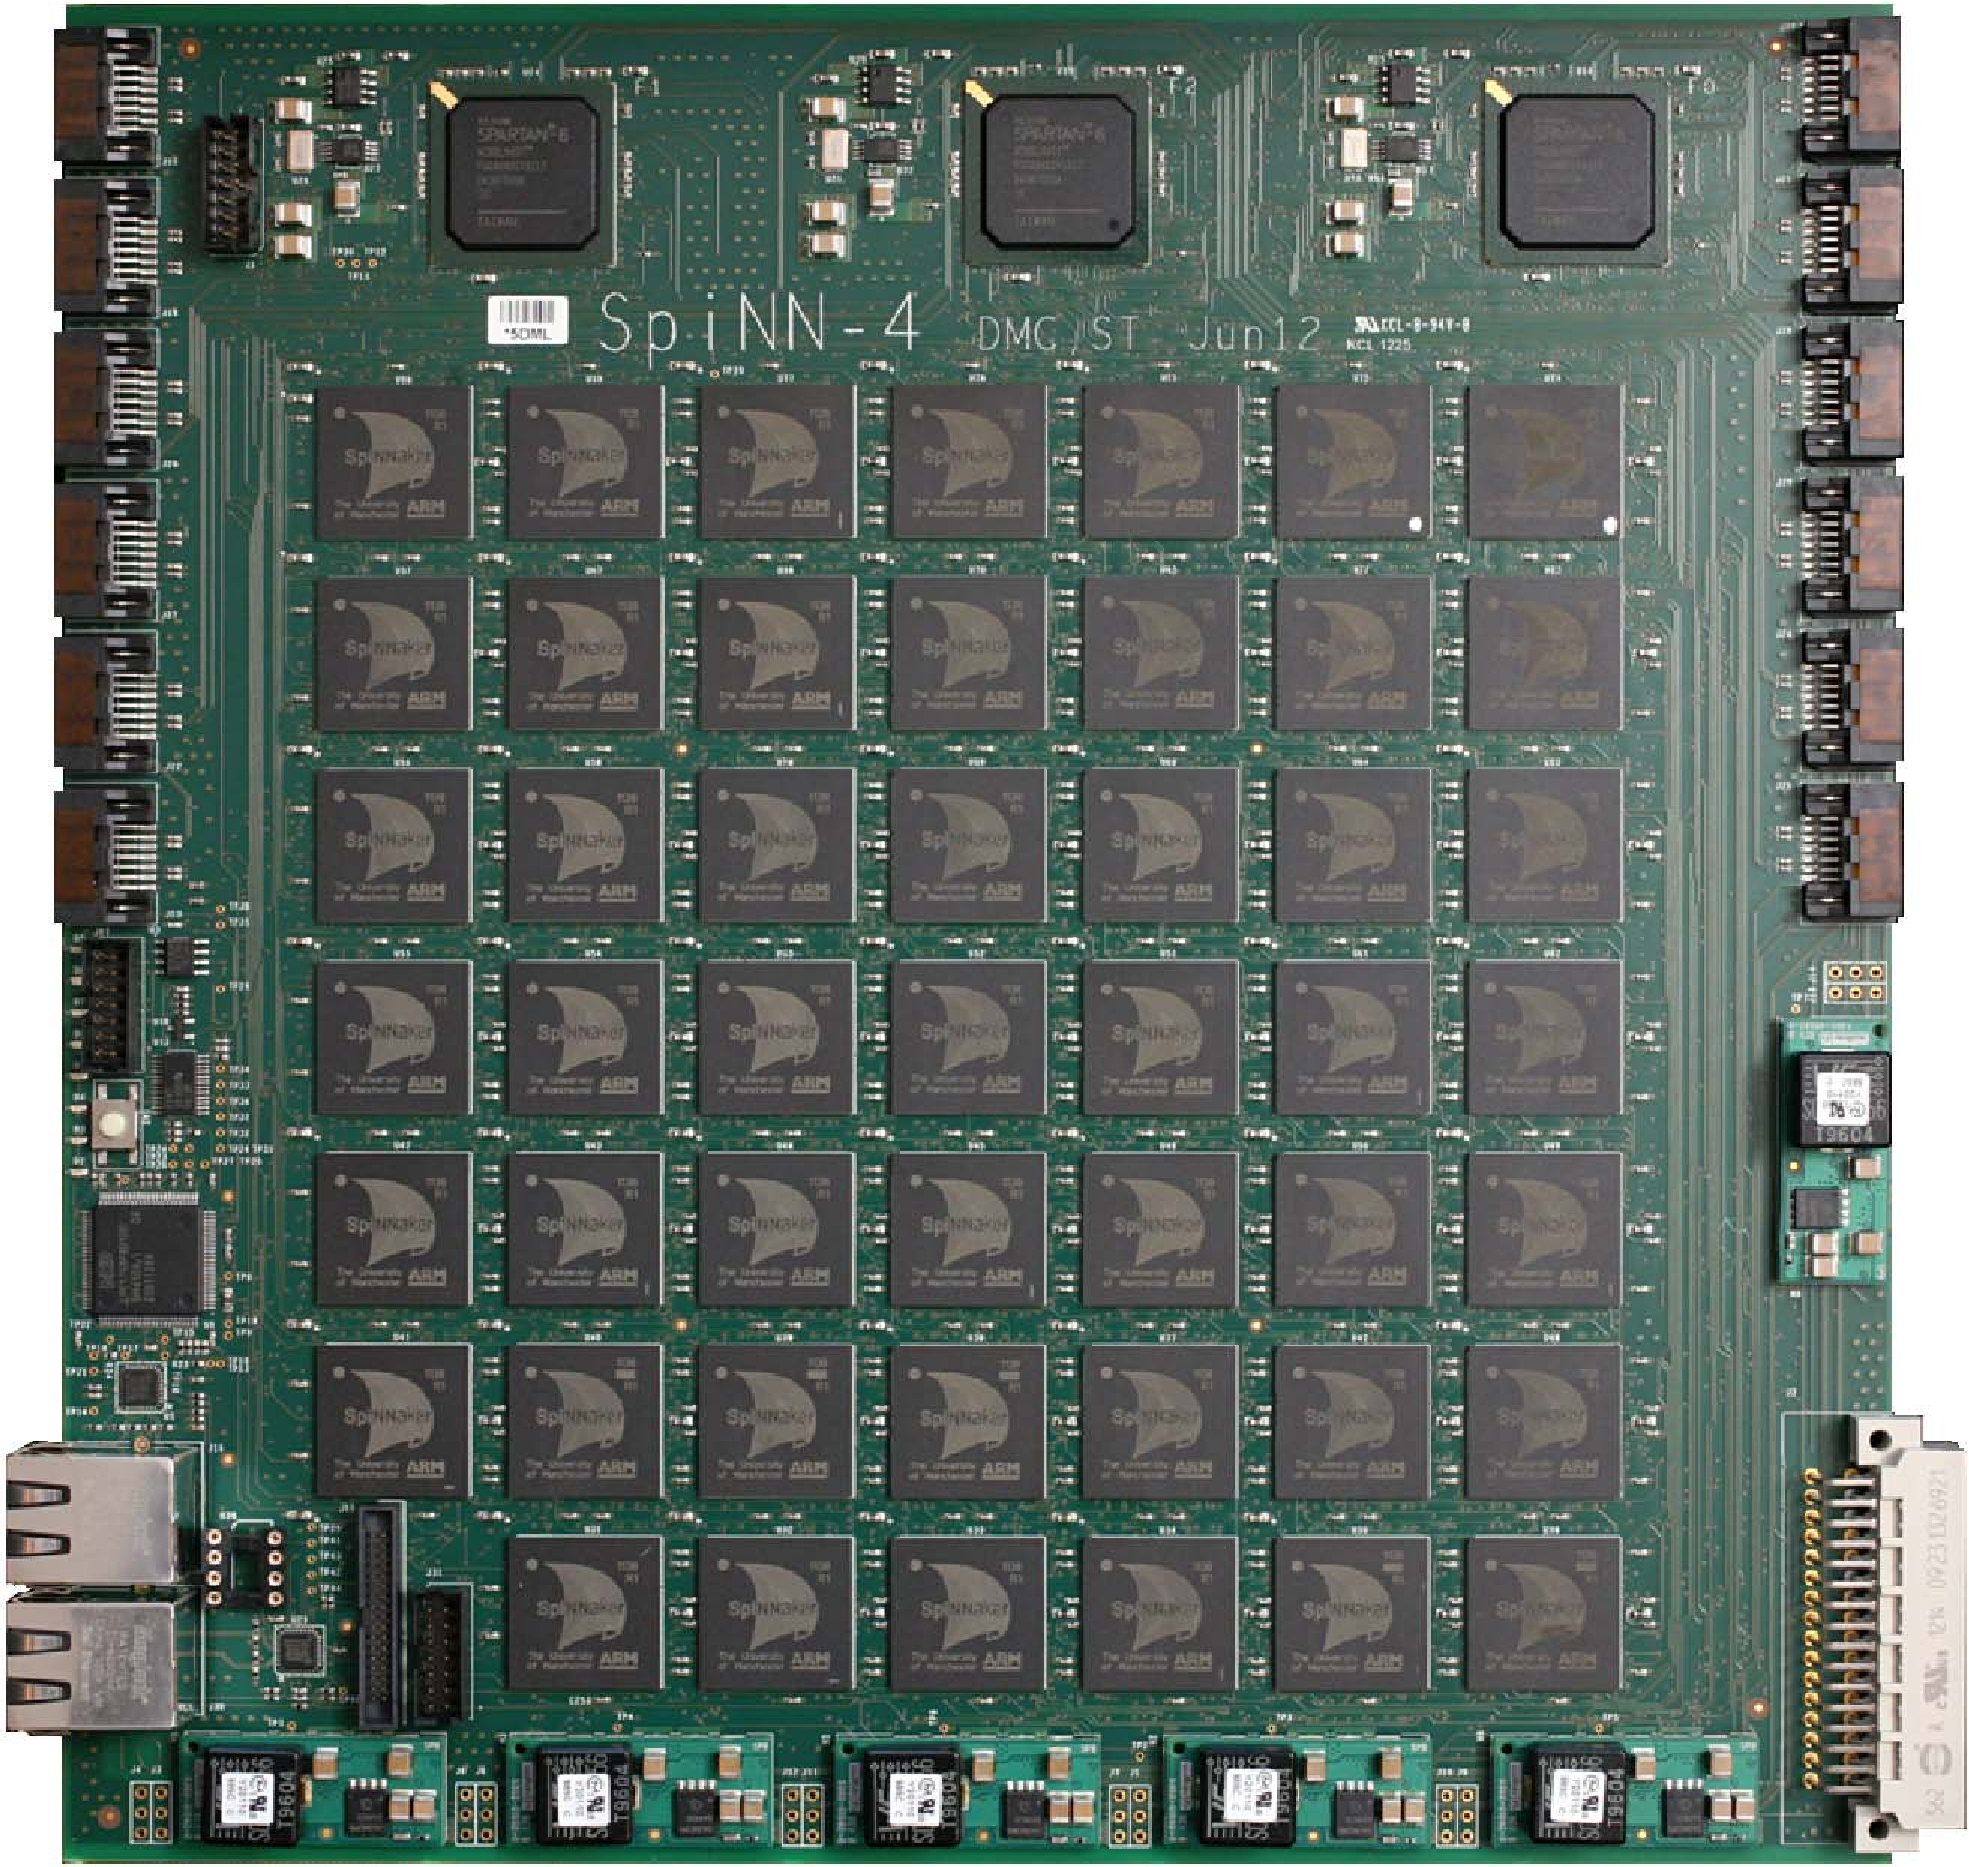
\includegraphics[width=0.6\textwidth]{pics/48node_pcb_resolution-white.pdf}
	\caption{103 Machine PCB}
	\label{fig:48node}
\end{figure}


\subsection{SpiNNaker distinguishing features}
Interfacing AER Sensors: 

Spikes from the silicon retina are injected to SpiNNaker through one of the 6 bi-directional on-board links by a SPARTAN-6 FPGA board that translates them into a SpiNNaker compatible AER format \footnote{AppNote 8 - Interfacing AER devices to SpiNNaker using an FPGA.}. 
From the software point of view, interfacing the silicon retina can be done using pyNN. 
The user sets a Spike Source population that resides on a virtual SpiNNaker chip, to which an AER sensor's spikes are directed, thus abstracting away the hardware details from the users\cite{galluppi2012real}.
